\documentclass[a4paper,12pt]{article}

\usepackage{fullpage} % Package to use full page
\usepackage{parskip} % Package to tweak paragraph skipping
\usepackage{amsmath}
\usepackage{hyperref}
\usepackage{amsmath,amsfonts,amsthm} % Math packages
\usepackage{graphicx}
\usepackage{listings}
\usepackage{color}
\usepackage{float}
\definecolor{codegreen}{rgb}{0,0.6,0}
\definecolor{codegray}{rgb}{0.5,0.5,0.5}
\definecolor{codepurple}{rgb}{0.58,0,0.82}
\definecolor{backcolour}{rgb}{0.95,0.95,0.92}
\definecolor{brown}{rgb}{0.59, 0.29, 0.0}
\definecolor{beaublue}{rgb}{0.74, 0.83, 0.9}
\definecolor{orange}{rgb}{1.0, 0.5, 0.0}
\definecolor{darkslategray}{rgb}{0.18, 0.31, 0.31}
\def\Xint#1{\mathchoice
	{\XXint\displaystyle\textstyle{#1}}%
	{\XXint\textstyle\scriptstyle{#1}}%
	{\XXint\scriptstyle\scriptscriptstyle{#1}}%
	{\XXint\scriptscriptstyle\scriptscriptstyle{#1}}%
	\!\int}
\def\XXint#1#2#3{{\setbox0=\hbox{$#1{#2#3}{\int}$}
		\vcenter{\hbox{$#2#3$}}\kern-.5\wd0}}
\def\dashint{\Xint-}

% Swap the definition of \abs* and \norm*, so that \abs
% and \norm resizes the size of the brackets, and the 
% starred version does not.
\makeatletter
\let\oldabs\abs
\def\abs{\@ifstar{\oldabs}{\oldabs*}}
%
\let\oldnorm\norm
\def\norm{\@ifstar{\oldnorm}{\oldnorm*}}
\makeatother
\definecolor{keywords}{RGB}{255,0,90}
\definecolor{comments}{RGB}{0,0,113}
\definecolor{red}{RGB}{160,0,0}
\definecolor{green}{RGB}{0,150,0}
\definecolor{codegreen}{rgb}{0,0.6,0}
\definecolor{codegray}{rgb}{0.5,0.5,0.5}
\definecolor{codepurple}{rgb}{0.58,0,0.82}
\definecolor{backcolour}{rgb}{0.95,0.95,0.92}
\definecolor{brown}{rgb}{0.59, 0.29, 0.0}
\definecolor{beaublue}{rgb}{0.74, 0.83, 0.9}
\definecolor{orange}{rgb}{1.0, 0.5, 0.0}
\definecolor{darkslategray}{rgb}{0.18, 0.31, 0.31}
\definecolor{deepblue}{rgb}{0,0,0.5}
\definecolor{deepred}{rgb}{0.6,0,0}
\definecolor{deepgreen}{rgb}{0,0.5,0}
\lstdefinestyle{myMatlabstyle}{
	language=Matlab,
	backgroundcolor=\color{white},   
	commentstyle=\color{codegreen},
	keywordstyle=\color{blue},
	identifierstyle=\color{brown},
	numberstyle=\tiny\color{codegray},
	stringstyle=\color{orange},
	basicstyle=\footnotesize,
	breakatwhitespace=false,         
	breaklines=true,                 
	captionpos=b,                    
	keepspaces=true,                 
	numbers=left,                    
	numbersep=5pt,                  
	showspaces=false,                
	showstringspaces=false,
	showtabs=false,                  
	tabsize=2
}
\lstdefinestyle{myPythonstyle}{
	language=Python, 
	basicstyle=\ttfamily\small, 
	keywordstyle=\color{blue},
	commentstyle=\color{green},
	stringstyle=\color{red},
	showstringspaces=false,
	identifierstyle=\color{black},
}
\lstset{language=Matlab,frame=single}
\lstset{language=Python,frame=single}

\title{AMATH 575: Problem Set 2}
\author{Jithin D. George, No. 1622555}
%\date{23/11/16}
% matrix environment
\newenvironment{mat}{\left[ \begin{array}{ccccccccccccc}}{\end{array}\right]}
\newcommand\bcm{\begin{mat}}
	\newcommand\ecm{\end{mat}}

\begin{document}

\maketitle
\begin{enumerate}

	
	\item 
	The vector field is given by 
	\[v'=-v\]
	\[\theta' =1 \]
	If our initial value of v is 0, it will remain 0 while theta changes continuously. This leads to a periodic orbit on the cylinder.
	
	The Bendixson theorem requires a simply connected domain. A cylinder has a hole in it and is far from simply connected. So, the theorem is not violated.
	
\item 
\begin{enumerate}
	\item
	The fixed points are at (0,0,0), (0,1,0),(0,0,1)and (1,0,0).
	The Jacobian is of the form 
	\[\bcm 0 &k_1 m_3 &k_2 m_2 \\ k_3 m_3 &0 &- k_1 m_1 \\ k_4 m_2 &k_5 m_1 &0\ecm \]
	where the ks are positive constants.
	For (0,0,0), all eigenvalues are 0. We cannot say anything about the stability.
	For (1,0,0), the Jacobian is 
	\[\bcm 0 &0 &0 \\ 0 &0 &- k_1 m_1 \\ 0 &k_5 m_1 &0\ecm \]
	
	We have two imaginary eigenvalues and 0(Mathematica). We cannot say anything about the stability.
	For (0,1,0), the Jacobian is 
	\[\bcm 0 &0 &k_2 m_2 \\ 0 &0 &0 \\ k_4 m_2 &0 &0\ecm \]
	
	We have two real eigenvalues and 0(Mathematica). One of the real eigenvalues is positive, indicating an unstable fixed point.
For (0,0,1), the Jacobian is 
\[\bcm 0 &k_1 m_3 &0 \\ k_3m_3 &0 &0 \\ 0 &0 &0\ecm \]

Again, we have two real eigenvalues and 0(Mathematica). One of the real eigenvalues is positive, indicating an unstable fixed point.
	
	\item 
	
	\[\dot{H}= \bigg[\frac{m_1 \dot{m_1}}{I_1}+ \frac{m_2 \dot{m_2}}{I_2}+\frac{m_3 \dot{m_3}}{I_3} \bigg] = \frac{m_1 m_2 m_3}{I_1 I_2 I_3}(I_2-I_3 +I_3-I_1+I_1-I_2)  =0 \]
	
	\[\dot{L}= 2m_1 \dot{m_1} +2m_2 \dot{m_2} + 2m_3 \dot{m_3}\] \[=2m_1m_2m_3\bigg[\frac{I_2-I_3}{I_2I_3}+ \frac{I_3-I_1}{I_1I_3} +\frac{I_1-I_2}{I_1I_2} \bigg]\] \[=2m_1m_2m_3\bigg[\frac{1}{I_3}- \frac{1}{I_2}+\frac{1}{I_1} - \frac{1}{I_3}+ \frac{1}{I_2} -\frac{1}{I_1} \bigg]\]
	\[ =0\]
\item
Using the following code, we plot the curves for initial conditions of different L values.
\begin{lstlisting}[style=MyPythonstyle]
import matplotlib as mpl
from mpl_toolkits.mplot3d import Axes3D
import numpy as np
import matplotlib.pyplot as plt

def d_stepper(v,f, steps,dt=0.05):
	fig = plt.figure()
	ax = fig.gca(projection='3d')
	z = np.zeros(steps)
	x = np.zeros(steps)
	y = np.zeros(steps)
	for k in v:
	z = np.zeros(steps+1)
	x = np.zeros(steps+1)
	y = np.zeros(steps+1)
	x[0]=k[0]
	y[0]=k[1]
	z[0]=k[2]
	for i in range(0,steps):
		x[i+1]= x[i]+dt*f(x[i],y[i],z[i])[0]
		y[i+1]= y[i]+dt*f(x[i],y[i],z[i])[1]
		z[i+1]= z[i]+dt*f(x[i],y[i],z[i])[2]
		ax.plot(x, y, z)
	plt.show()

def q_532(x,y,z):
	f= (1/6)*y*z
	g= (-3/10)*x*z
	h= (2/15)*x*y
	return [f,g,h]
	
d_stepper([[1,1,1],[2,2,2],[1,1,2] ,[2,2,1], ],q_532,600)	
\end{lstlisting}
\begin{figure}[H] 
	\centering
	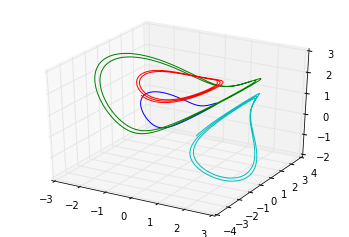
\includegraphics[width=10cm]{Lspace}
	\caption{Orbits for L=3, 12, 6 and 9 }
\end{figure}

A single L value would look like the figure below
\begin{figure}[H] 
	\centering
	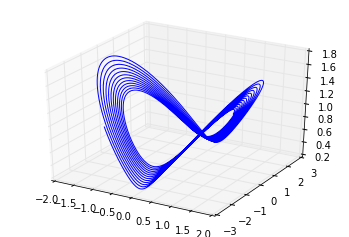
\includegraphics[width=10cm]{singleL}
	\caption{Orbits for L=3 }
\end{figure}
\end{enumerate}


	
	\item
	\begin{enumerate}
		\item 
		We attempt a proof by contradiction.
		\[J_1 = \sum_{k=1}^{N}x_k\]
		For N=1,
			\[J_1 = x_1\]
			\[J_1'= x_1' = 0\]
			
	For N=w,
	we assume
\[ J_1' = \sum_{k=1}^{w}x_k' = 0\]

For N= w+1,
\[ J_1' = \sum_{k=1}^{w+1}x_k' = \sum_{k=1}^{w}x_k' +  \sum_{k=1}^{w} \frac{-2v}{x_k -x_{w+1}} +  \sum_{k=1}^{w} \frac{-2v}{x_{w+1}-x_{k} } \]
\[ = 0 +  -2v\sum_{k=1}^{w} \bigg[\frac{1}{x_k -x_{w+1}} -  \frac{1}{x_{k}-x_{w+1} }\bigg] = 0 \]

Thus, by induction, we have proved $J_1$ is a conserved quantity.

\item 
We attempt a proof by contradiction.
\[J_2 = \frac{1}{2}\sum_{k=1}^{N}x_k^2 + vN(N-1)t\]
For N=1,
\[J_2 = \frac{1}{2}x_1^2 \]
\[J_2'= x_1 x_1' = 0\]

For N=w,
we assume
\[ J_2' = \sum_{k=1}^{w}x_k x_k' + vw(w-1) = 0\]

For N= w+1,
\[ J_2' = \sum_{k=1}^{w+1}x_k x_k' + v(w+1)w \]\[ = \sum_{k=1}^{w+1}x_k x_k' + vw(w-1)+2vw\]
\[ = \sum_{k=1}^{w}x_kx_k' +  \sum_{k=1}^{w} \frac{-2vx_k}{x_k -x_{w+1}} +  \sum_{k=1}^{w} \frac{-2vx_{w+1}}{x_{w+1}-x_{k} } + vw(w-1)+2vw\]
\[ = \sum_{k=1}^{w}x_kx_k'  + vw(w-1) +  \sum_{k=1}^{w} \frac{-2vx_k}{x_k -x_{w+1}} +  \sum_{k=1}^{w} \frac{2vx_{w+1}}{x_k -x_{w+1} } +2vw\]
\[= 0 -  \sum_{k=1}^{w} \frac{-2vx_{w+1}+2vx_k}{x_k -x_{w+1} } +2vw \]
\[= 0 -  \sum_{k=1}^{w} 2v +2vw \]
\[=-2vw+2vw =0\]
Thus, by induction, we have proved $J_2$ is a conserved quantity.
		
	\end{enumerate}
	\item
	Although an integral is introduced as being tangent to a flow, its defining property is that it is constant along the flow.
	Thus, a function that remains the same along the orbit of a map is the equivalent of an integral for a map.
	Thus, if f is the function that defines the map on x, \[I(x_0)= I(f(x_0))= I(f^n(x_0)), \text{ for any n}\]
		\item
		For the Lorenz equations,
		\[\nabla . f = \frac{\partial f}{\partial x} + \frac{\partial f}{\partial y} + \frac{\partial f}{\partial z}= -\sigma -1 - \beta  = -r \]
		where r is a positive constant
		So, we have 
		\[\frac{dV}{dt}= \int_{D_0}-r dx \]
		\[\frac{dV}{dt}= -r V \]
		\[V= V_0 e^{-rt}\]
		
		Thus, for the Lorenz equation, the volume shrinks with time.
\item
\[\theta_{n+1} = \theta_{n} + I_n - \frac{1}{2\pi}sin2\pi\theta_{n} \text{ mod } 1\]
\[I_{n+1} =  I_n - \frac{K}{2\pi}sin2\pi\theta_{n} \]
For $(\theta,I)= (1/2,1)$,
\[\theta_{n+1} = \theta_{n} +1- \frac{1}{2\pi}sin\pi \text{ mod } 1=  \theta_{n} +1 \text{ mod } 1 = \theta_{n}\]
\[I_{n+1} =  I_n - \frac{1}{2\pi}sin\pi=I_n  \]

Thus,  $(\theta,I)= (1/2,1)$ is a fixed point.
The Jacobian at this point is given by 
\[ \bcm 2 & 1  \\  1 & 1 \ecm \] 

The eigenvalues are $\frac{3+ \sqrt{5}}{2}$ and $\frac{3- \sqrt{5}}{2}$ meaning one stable manifold and one unstable manifold. We find the corresponding eigenvectors($(0.5+ 0.5*(1+\sqrt(5)),1)$ and $(0.5+ 0.5*(1-\sqrt(5)),1)$) and construct the homoclinic tangle.

The inverse map is given by
\[\theta_{n} = \theta_{n+1} - I_{n+1}  \text{ mod } 1\]
\[  I_n =I_{n+1} + \frac{K}{2\pi}sin2\pi\theta_{n} \]



\begin{lstlisting}[style=MyPythonstyle]
"""
MapStepper:

Steps through maps forward and backward in time
Created on Sun Apr 23 17:09:22 2017

@author: Jithin
"""
import numpy as np
import matplotlib.pyplot as plt




def mapstandard(u, steps =19,dt =1):
	marray = np.zeros((steps+1,2))
	for i in [0,1]:
		marray[0,i]= u[i]
		for i in range(1,steps+1):            
		marray[i,1]= array[i-1,1]
		-dt*(1/(2*np.pi))*np.sin(2*np.pi*marray[i-1,0])
		if dt ==1:
		marray[i,0]= (marray[i-1,0] +marray[i-1,1]-(1/(2*np.pi))*np.sin(2*np.pi*marray[i-1,0]))%1
		marray[i,1]= marray[i-1,1] -dt*(1/(2*np.pi))*np.sin(2*np.pi*marray[i-1,0])
		else:
		marray[i,0]= (marray[i-1,0] - marray[i-1,1] )%1
		marray[i,1]= marray[i-1,1] -dt*(1/(2*np.pi))*np.sin(2*np.pi*marray[i,0])
	return marray

def poltt(dx):
	a= 0.5+ 0.5*(1+np.sqrt(5))*dx
	b= 1+dx*1
	c= 0.5+ 0.5*(1-np.sqrt(5))*dx
	d= 1+dx*1
	return [a,b],[c,d]

def plotline():
	a = np.linspace(-0.0000001,0.0000001,100)
	for dx in a:
		w1,w2 =poltt(dx)
		q2= mapstandard(w2,20,-1)
		lo =plt.scatter(q2[:,0],q2[:,1],s=5,color='r')
	a = np.linspace(-0.0000001,0.0000001,100)
	for dx in a:
		w1,w2 =poltt(dx)
		q= mapstandard(w1,20)
		ll=plt.scatter(q[:,0],q[:,1],s=5)
	dx=0.00000000001
	w1,w2 =poltt(dx)
	q3= mapstandard(w1,150,1)
	lw =plt.plot(q3[:,0],q3[:,1],'g', label='The orbit')
	plt.legend((lo, ll,lw),('The stable manifold',
	 'The unstable manifold','The orbit'),loc='lower left', 
	 fontsize=8)
	plt.show

plotline()  
\end{lstlisting}
\begin{figure}[H] 
	\centering
	\includegraphics[width=12cm]{standardmap}
	\caption{Stable, unstable manifolds and an orbit }
\end{figure}

Here, the red line is the stable manifold, blue the unstable and green is the orbit.
 
\item	

\[\dot{x} = -x +ay + x^2y \]
\[\dot{y} =  b - ay - x^2y \]
Setting the equations above to zero, we have
\[y = \frac{x}{a+x^2} \text{ and } y = \frac{b}{a+x^2}\]
This implies a fixed point at $(b,\frac{b}{a+b^2})$. If the fixed point is unstable, it would be a perfect candidate to construct the trapping region around. By Poincare-Bendixson, if the trapping region has no flows outward and if the only fixed point inside is not an attractor (thus being a limit point), the only possible alternatives for limit sets are periodic orbits.

But for that the fixed point has to be unstable. The Jacobian at th fixed point is given by 
\[ \bcm 1+\frac{2b^2}{a+b^2} & a+b^2\\-\frac{2b^2}{a+b^2} &-a-b^2\ecm\]

The eigenvalues end looking very complicated.
We instead look at the trace. If the trace is greater than 0, the fixed point is unstable.

Using Mathematica, we find the trace to be
\[- \frac{a^2 +2ab^2-a +b^4- 3b^2}{a + b^2}  \] 
We need this to be greater than 0.

Mathematica yields
\[b = \sqrt{0.5(1-2*a \pm \sqrt{1-8a})}\]
The nifty code below plot the range of b for a and whether it is stable or unstable. 
\begin{lstlisting}[style=MyPythonstyle]
import numpy as np
import matplotlib.pyplot as plt

asp = np.linspace(0,1/8,1000)

for a in asp:
	j = np.sqrt(0.5*(1-2*a-np.sqrt(1-8*a)))
	plt.plot(a,j,'bo')
	w = np.sqrt(0.5*(1-2*a+np.sqrt(1-8*a)))
	plt.plot(a,w,'bo')

plt.show	
\end{lstlisting}

\begin{figure}[H] 
	\centering
	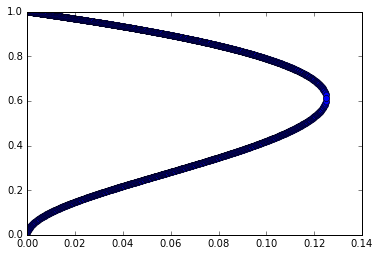
\includegraphics[width=10cm]{trap}
	\caption{Stable regions for b }
\end{figure}

Simple calculations lead to which regions are stable.

Now, to find the trapping regions.

We plot the nullclines to see the direction of flows.
The nullclines are given by
\[\dot{x}= \frac{b}{a+x^2}\]
\[\dot{y}= \frac{x}{a+x^2}\]

\begin{figure}[H] 
	\centering
	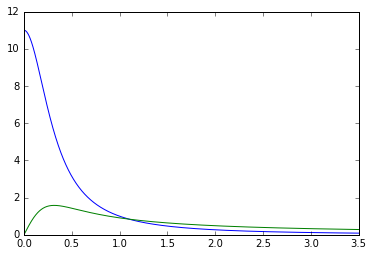
\includegraphics[width=10cm]{xdot}
	\caption{Nullclines }
\end{figure}
A regular big box would not be good enough. We see that $\dot{x}>0$. So, we need a slanted boundary because the flow would not go inside if it is a vertical line. The flow inwards along y should be greater than the flow outside along x creating a new vector of inward flow.

Thus, we need
\[ \dot{y} < - \dot{x}\] 
\[ \dot{y} + \dot{x}<0\] 
\[-x+b<0\]

So, for the slanted line,
\[x>b\]

\begin{figure}[H] 
	\centering
	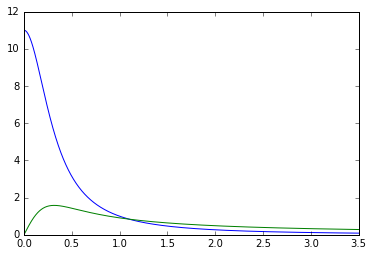
\includegraphics[width=10cm]{xdot}
	\caption{The box }
\end{figure}

	\end{enumerate} 
\end{document}